\documentclass[a4paper, 11pt]{article}
\usepackage{../preamble}

\begin{document}

\doctype{Practical Work}
\coursetitle{Graphs in Machine Learning}
\semester{MVA Fall 2019}
\instructor{Michal Valko}
\teachingassistant{Omar Darwiche-Domingues, Pierre Perrault}
\student{Antoine Moulin}
\worknumber{2}
\workdate{November 12}

\maketitle

\vspace*{1.5cm}

The report and the code are due in 2 weeks (deadline 23:59 26/11/2019). You will find instructions on how to submit the report on piazza, as well as the policies for scoring and late submissions. All the code related to the TD must be submitted.

% -------------------------------------------------------------------
\section{Harmonic Function Solution (HSF)}

\begin{enumerate}
	\item \textbf{Complete \path{hard_hfs} and \path{two_moons_hfs}. Select uniformly at random 4 labels ($S$), and compute the labels for the unlabeled nodes ($T$) using the hard-HFS formula. Plot the resulting labeling and the accuracy.}
	
    The Laplacian matrix and the vector $f$ can be written specifying the labeled and unlabeled parts as follow:
    
    \begin{equation*}
        \mathbf{L} = \begin{pmatrix}
            \mathbf{L}_{ll} & \mathbf{L}_{lu} \\
            \mathbf{L}_{ul} & \mathbf{L}_{uu}
        \end{pmatrix}
        \hspace*{.5cm}
        \mathbf{f} = \begin{pmatrix}
            \mathbf{f}_{l} \\
            \mathbf{f}_{u}
        \end{pmatrix}
    \end{equation*}
	
	As shown in class, when computing the hard HFS, one can use the formula:
	
	\begin{equation*}
	    \mathbf{f_{u}} = - \mathbf{L_{uu}^{+}} \mathbf{L_{ul}} \mathbf{f_{l}}
	\end{equation*}
	
	where $\mathbf{L_{uu}^{+}}$ is the Moore-Penrose inverse of $\mathbf{L_{uu}}$, in case the matrix is not invertible. Let's use a $12$-nn graph and the normalized Laplacian $\mathbf{L}_{rw}$. The results are shown in figure \ref{fig:q11-hard-hfs}. \\
	
	\begin{figure*}[!htb]
	    \centering
	    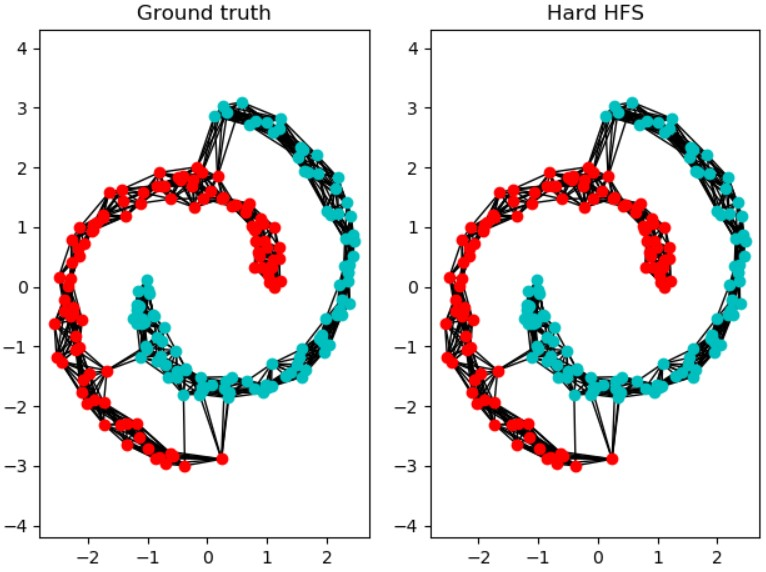
\includegraphics[width=.5\textwidth]{images/q11_hard-hfs.jpg}
	    \caption{HFS with $12$-nn graph and $L_{rw}$ Laplacian (without regularization). The resulting accuracy is $1$.}
	    \label{fig:q11-hard-hfs}
	\end{figure*}
	
	\item \textbf{At home, run \path{two_moons_hfs} using the \path{data_2moons_large.mat}, a dataset with 1000 samples. Continue to uniformly sample only 4 labels. What can go wrong?}
	
	When using a larger dataset, there is a larger probability of sampling four examples from the same class and thus generate many errors. Here, in most of the cases it works well, but sometimes, it is possible to have results as shown in figure \ref{fig:q12-hard-hfs-fail}, where the accuracy is $0.5$.
	
	\begin{figure*}[!htb]
	    \centering
	    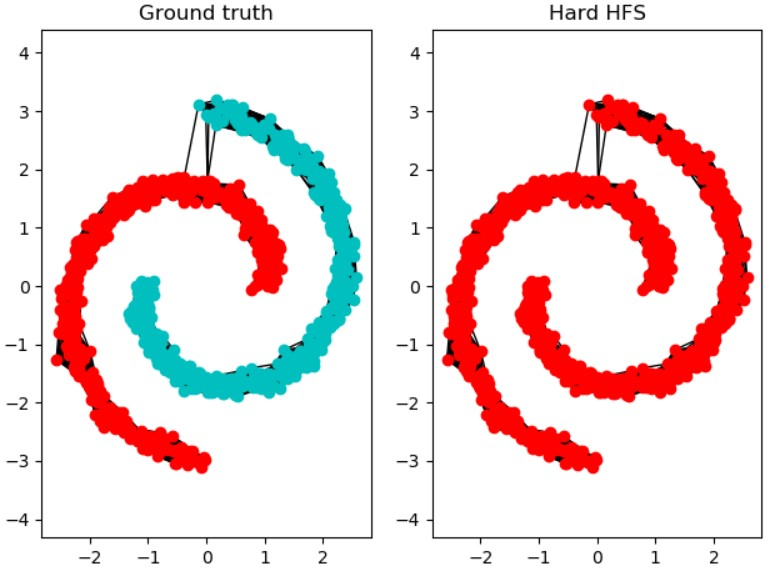
\includegraphics[width=.5\textwidth]{images/q12_hard-hfs-fail.jpg}
	    \caption{HFS with $40$-nn graph and $L_{rw}$ Laplacian (without regularization). The resulting accuracy is $0.5$.}
	    \label{fig:q12-hard-hfs-fail}
	\end{figure*}
	
	\item \textbf{Complete \path{soft_hfs} and test it with \path{two_moons_hfs}. Now complete \path{hard_vs_soft_hfs}. Compare the results you obtain with soft-HFS and hard-HFS.}
	
	Let's test the soft HFS method. We make sure that the labeled examples are more important than the unlabeled ones, and we fix $c_l = 0.9$ and $c_u = 0.1$. In figure \ref{fig:q13-soft-hfs}, one can see that the results achieved by soft HFS on the two-moons dataset are as good as with hard HFS.
	
	\begin{figure*}[!htb]
	    \centering
	    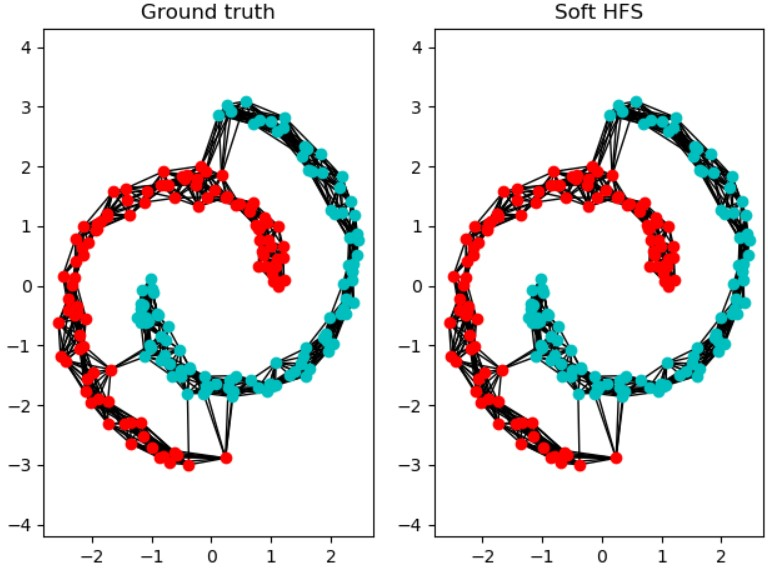
\includegraphics[width=.5\textwidth]{images/q13_soft-hfs.jpg}
	    \caption{Soft HFS with $12$-nn graph and $L_{rw}$ Laplacian (without regularization). The parameters regarding the respective importance of labeled and unlabeled examples are: $c_l = 0.9, c_u = 0.1$. The resulting accuracy is $1$.}
	    \label{fig:q13-soft-hfs}
	\end{figure*}
	
	Now, let's compare both methods with the function \texttt{hard\_vs\_soft\_hfs}. This time, the constants $c_l$ and $c_u$ are fixed to $0.95$ and $0.05$, respectively. When running the function several times, we see that on average, soft HFS seems to perform better than hard HFS, even though the difference is very small. For instance, with $10$ measures, we get an accuracy of $0.8785$ (standard deviation: $0.068$) for hard HFS and an accuracy of $0.8815$ (standard deviation: 0.067) for soft HFS. The results are shown in figure \ref{fig:q13-comparison}. We could think that with a much larger dataset, this difference would be larger as well, hence showing that with noisy examples, it is better to use soft HFS to avoid propagating too many errors.
	
	\begin{figure*}[!htb]
	    \centering
	    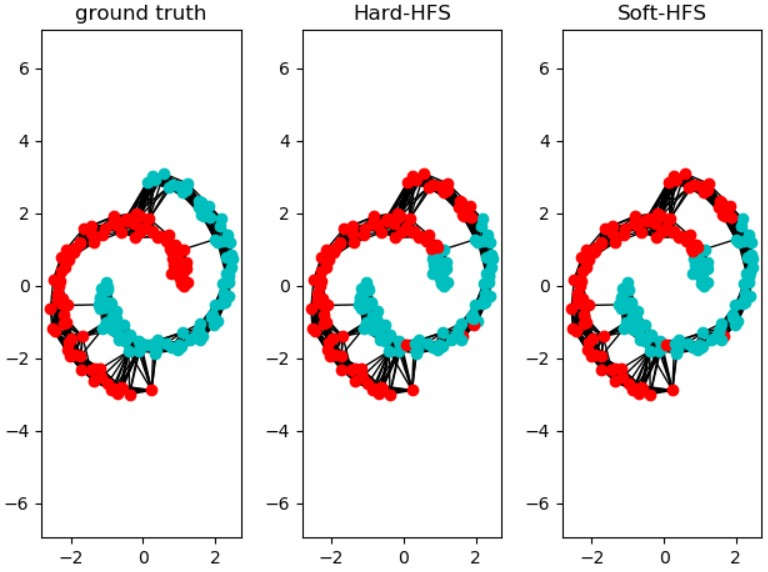
\includegraphics[width=.5\textwidth]{images/q13_comparison.jpg}
	    \caption{$12$-nn graph and $L_{rw}$ Laplacian (without regularization). The parameters regarding the respective importance of labeled and unlabeled examples (for soft HFS) are: $c_l = 0.95, c_u = 0.05$.}
	    \label{fig:q13-comparison}
	\end{figure*}
\end{enumerate}

\pagebreak
% -------------------------------------------------------------------
\section{Face recognition with HFS}

In figure \ref{fig:small-faces-dataset} is shown the small dataset on which is first used HFS.

\begin{figure}[!htb]
    \centering
    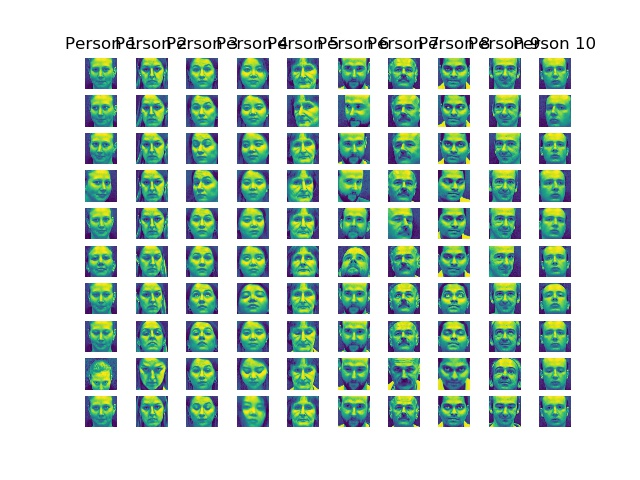
\includegraphics[width=.6\textwidth]{images/faces_dataset.jpg}
    \caption{The dataset contains $10$ photos of $10$ different faces.}
    \label{fig:small-faces-dataset}
\end{figure}

\begin{enumerate}
	\item \textbf{How did you manage to label more than two classes?}
	
	When dealing with more than two classes, one can turn the labels into one-hot vectors, \ie vectors whose components are $0$ except at the index of the class, where it is $1$ (e.g. an example with class $1$ would be associated to $[0, 1]$). Hence, the HFS solution $\mathbf{f}$ that previously belonged to $\R^{N}$ now belongs to $\R^{N \times C}$ where $C$ is the number of classes.
	
	\item \textbf{Which preprocessing steps (e.g. cv.GaussianBlur, cv.equalizeHist) did you apply to the faces before constructing the similarity graph? Which gave the best performance?}
	
	At first, I tried the following procedure: convert the image from RGB to HSL, apply histogram equalization on one of the channels (I first wanted to try on the lightness channel but I also tried the others), convert the image from HSL to RGB and then to grayscale, apply a median filter and then normalize the image. The idea of applying histogram equalization in the HSL space comes from a previous project I did.
	
	But the results were very similar to the ones obtained with: convert from RGB to grayscale, apply a histogram equalization, apply a median filter and normalize. Hence, it was not really useful. 
	
	Finally, I discovered the function \texttt{cv2.createCLAHE}, which applies an adaptive histogram equalization (explained here: \url{https://docs.opencv.org/master/d5/daf/tutorial_py_histogram_equalization.html} ; in brief, it applies histogram equalization locally so information is not lost due to over-brightness) which gives better results than my first attempt. So I apply the second idea with an adaptive histogram equalization instead of the usual one.
	A result is shown in figure \ref{fig:q22-results}.
	
	\begin{figure}
	    \centering
	    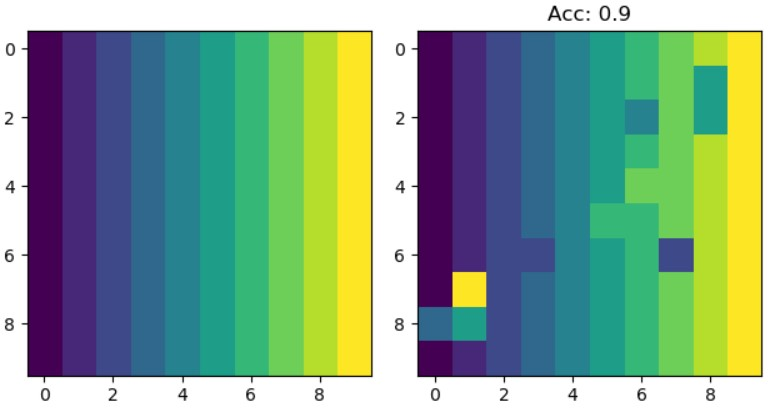
\includegraphics[width=.6\textwidth]{images/q22_results}
	    \caption{Results of the face recognition algorithm.}
	    \label{fig:q22-results}
	\end{figure}
	
	\item \textbf{Does HFS reach good performances on this task?}
	
	On an average of $10$ measures, we see that HFS can reach an accuracy of $0.87$ (with a standard deviation of $0.013$). Today, there are some models (e.g. deep neural networks) that can reach $0.99$ accuracy. Hence, HFS is not excellent when we compare it to such models, but it is possible that a better preprocessing could improve the performances. Besides, compared to the training required to reach these performances, it is very good.
	
	\item \textbf{Did adding more data to the task improve performance? If so, which kind of additional data improves performance?}
	
	Adding more unlabeled data to the task did not improve performance. On an average of $10$ measures, the accuracy obtained is $0.60$ (with a standard deviation of $0.043$). A result is shown in figure \ref{fig:q24-results}. But adding labeled examples would improve performance (besides the fact that it adds an example that is to be well classified, it will also help classifying other examples).

	\begin{figure}[!htb]
	    \centering
	    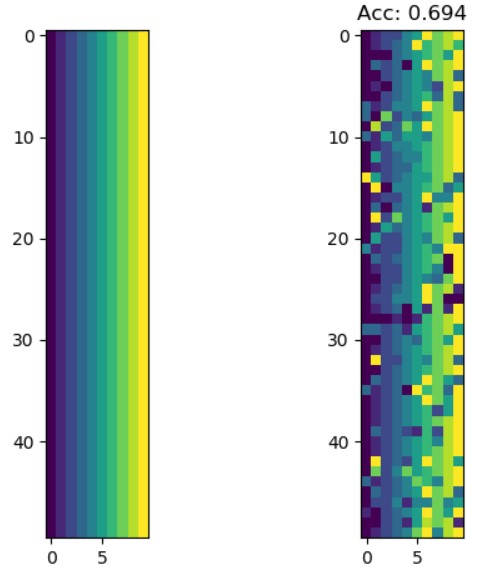
\includegraphics[width=.3\textwidth]{images/q24_results}
	    \caption{Results of the face recognition algorithm.}
	    \label{fig:q24-results}
	\end{figure}
	
	\item \textbf{If the performance does not improve when including additional data, try to justify why. Which kind of additional data degrades performance instead of improving it?}
	
	We first note that in both cases, only $4$ labeled examples are provided by person. It means that in the first case, $40\%$ of the dataset is labeled, whereas in the second case, only $8\%$ of the dataset is labeled. Hence it may due to the fact that on this larger graph, errors can propagate more easily. Besides, if the new images have a poor quality, then it is likely to induce more errors than without these images.
	
\end{enumerate}

\pagebreak
% -------------------------------------------------------------------
\section{Online SSL}

\begin{enumerate}
	\item \textbf{Complete \path{online_ssl_update_centroids} using the pseudocode 1.}
    
    See the code.

	\item \textbf{Complete \path{online_ssl_compute_solution} following the pseudocode 2.}

    See the code.

	\item \textbf{Read the function \path{preprocess_face} (in \path{helper_online_ssl.py}) and run \path{online_face_recognition}. Include some of the resulting frames (not too similar)
	in the report showing faces correctly being labeled as opposite, and comment on the choices you made during the implementation.}
	
	In figure \ref{fig:ariane-antoine} is shown a photo in which the algorithm recognizes Ariane and I.
	
	\begin{figure}[!h]
	    \centering
	    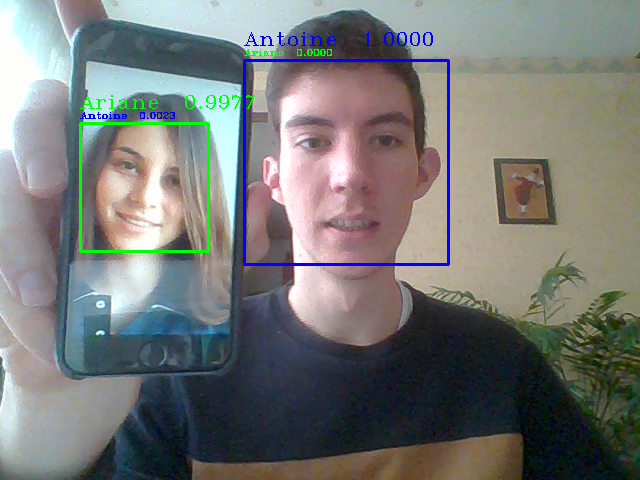
\includegraphics[width=.5\textwidth]{images/q33_ariane_antoine.png}
	    \caption{Photo of Ariane and Antoine being well classified by the algorithm.}
	    \label{fig:ariane-antoine}
	\end{figure}
	
	However, the algorithm is not really stable and it is not always easy to classify well the faces of Ariane and I. This may come from the fact that only $15$ images per person were used, or that the parameters were badly chosen. Besides, the adaptive histogram equalization made previously is not done here, because it yields bad performance.
	
	\item \textbf{What happens if an unknown person's face is captured by the camera? Modify your code to be able to disregard faces it cannot recognize,
	and include some of the resulting frames (not too similar) in the report showing unknown faces correctly being labeled as unknown.}
	
	An unknown person's face is often classified as Ariane or I. To solve this, it is possible to add a constraint on the vector $f$ and classify the face as unknown if the largest probability in the vector $f$ is less than a threshold, e.g. $0.9$. An example is shown in figure \ref{fig:marie-unknown}. This heuristic is very simple and a more robust way would be to compare the new face with the faces of the assigned class (or the centroid). For instance, if Marie's face is classified as Ariane, a simple comparison with a photo of Ariane would enable the algorithm to see that Marie is not Ariane.
	
	\begin{figure}[!h]
	    \centering
	    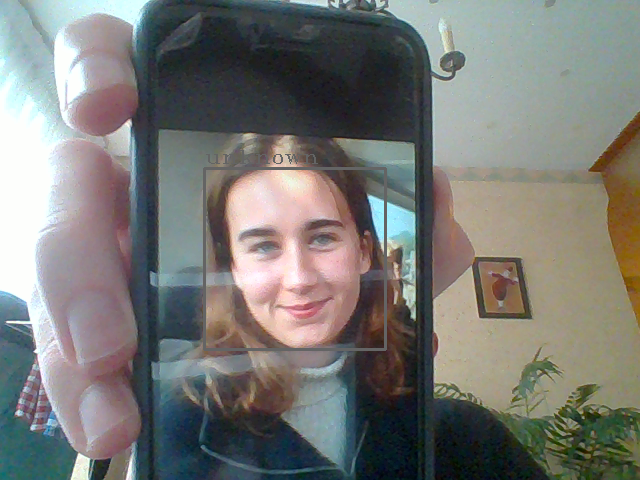
\includegraphics[width=.6\textwidth]{images/q34_marie_unknown.png}
	    \caption{A third person, Marie, is classified as unknown by the classifier.}
	    \label{fig:marie-unknown}
	\end{figure}
	
\end{enumerate}

\end{document}